% 图 4：闭环负反馈框图
\documentclass[border=6pt]{standalone}
% 四张示意图共用的字体、颜色与 TikZ 设置
\usepackage{fontspec}
\usepackage{xeCJK}
\setmainfont{TeX Gyre Pagella}
\setCJKmainfont{Noto Serif CJK SC}[AutoFakeSlant=0.15]
\usepackage{unicode-math}
\setmathfont{TeX Gyre Pagella Math}
\usepackage{amsmath}
\usepackage{tikz}
\usetikzlibrary{arrows.meta, positioning, calc, decorations.markings, backgrounds, fit, shapes.geometric}

\definecolor{navy}{HTML}{1E3A8A}
\definecolor{teal}{HTML}{0F766E}
\definecolor{amber}{HTML}{B45309}
\definecolor{softblue}{HTML}{EFF6FF}
\definecolor{softteal}{HTML}{F0FDFA}
\definecolor{softamber}{HTML}{FFFBEB}
\definecolor{border}{HTML}{CBD5E1}
\definecolor{graytext}{HTML}{5B6673}
\definecolor{redalert}{HTML}{991B1B}

\tikzset{
  >=Latex,
  every node/.style={font=\small},
  block/.style={draw=navy, thick, rounded corners=3pt, fill=softblue, align=center},
  bus/.style={thick, graytext},
}

\begin{document}
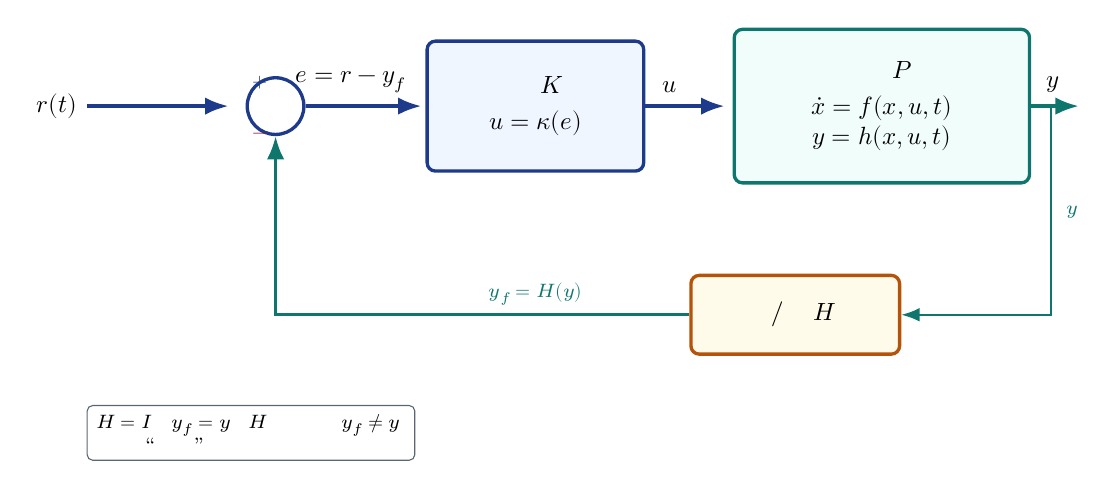
\begin{tikzpicture}[x=1cm,y=1cm]
  % 参考输入
  \node[anchor=east] (r) at (-1.25,2.0) {$r(t)$};
  \draw[->, very thick, navy] (r.east) -- (0.55,2.0);

  % 求和点
  \node[circle, draw=navy, very thick, fill=white, minimum size=0.72cm] (sum) at (1.15,2.0) {};
  \node[text=navy, font=\scriptsize] at (0.95,2.30) {$+$};
  \node[text=redalert, font=\scriptsize] at (0.95,1.62) {$-$};
  \node[text=redalert, font=\scriptsize, align=center] at (1.15,0.95) {负反馈求和点};

  % 误差 -> 控制器
  \draw[->, very thick, navy] (sum.east) -- (3.0,2.0);
  \node[above] at (2.10,2.05) {$e=r-y_f$};
  \node[draw=navy, very thick, rounded corners=3pt, fill=softblue, align=center,
        minimum width=2.75cm, minimum height=1.65cm] (K) at (4.45,2.0)
        {\textbf{控制器 $K$}\\[2pt]$u=\kappa(e)$};

  % 控制器 -> 被控对象
  \draw[->, very thick, navy] (K.east) -- (6.85,2.0);
  \node[above] at (6.15,2.05) {$u$};
  \node[draw=teal, very thick, rounded corners=3pt, fill=softteal, align=center,
        minimum width=3.75cm, minimum height=1.95cm] (P) at (8.85,2.0)
        {\textbf{被控对象 $P$}\\[2pt]$\dot x=f(x,u,t)$\\$y=h(x,u,t)$};

  % 输出
  \draw[->, very thick, teal] (P.east) -- (11.35,2.0);
  \node[above] at (11.02,2.05) {$y$};

  % 反馈通道：y -> 测量/传感器 H -> 求和点
  \draw[thick, teal] (11.00,2.0) -- (11.00,-0.65) -- (9.15,-0.65);
  \node[right, text=teal, font=\scriptsize] at (11.07,0.65) {$y$};
  \node[draw=amber, very thick, rounded corners=3pt, fill=softamber,
        minimum width=2.65cm, minimum height=1.0cm] (H) at (7.75,-0.65)
        {测量/传感器 $H$};
  \draw[->, thick, teal] (9.15,-0.65) -- (H.east);
  \draw[->, very thick, teal] (H.west) -- (1.15,-0.65) -- (sum.south);
  \node[above, text=teal, font=\scriptsize] at (4.45,-0.65) {$y_f=H(y)$};

  % 说明
  \node[draw=graytext, rounded corners=2pt, fill=white, align=left, font=\scriptsize,
        anchor=west] at (-1.25,-2.15)
    {$H=I$ 时 $y_f=y$；若 $H$ 含滤波、采样或估计，则 $y_f\ne y$。\\
     负号表示控制器依据“参考与反馈之差”动作。};
\end{tikzpicture}
\end{document}
